\documentclass[journal, 12pt, twocolumn]{IEEEtran}

\usepackage{amsmath}
\usepackage{graphicx}
\usepackage{enumitem}
\usepackage{listings}
\usepackage[justification=centering]{caption}

\lstset{
%language=C,
basicstyle=\ttfamily,
frame=single,
breaklines=true,
columns=fullflexible
}

\providecommand{\pr}[1]{\ensuremath{\Pr\left(#1\right)}}

\title{Random Numbers}
\author{Kartheek Tammana}
\date{\today}

\begin{document}

\maketitle

\section{Uniform Random Variables}
Let $U$ be a uniform random variable between 0 and 1.
\begin{enumerate}[label=\arabic{section}.\arabic*]
    \item
        Generate $10^6$ samples of $U$ using a C program and save into a file called uni.dat
        \\
        \textbf{Solution} Download the following C file.
        \begin{lstlisting}
wget https://raw.githubusercontent.com/kst164/AI1110-Assignments/main/rand_nums/codes/gen_uniform.c
        \end{lstlisting}
        And run it using
        \begin{lstlisting}
cc gen_uniform.c
./a.out > uni.dat
        \end{lstlisting}

    \item
        Load the uni.dat file into python and plot the empirical CDF of $U$ using the samples in uni.dat.
        \\
        \textbf{Solution} Download the following files.
        \begin{lstlisting}
wget https://raw.githubusercontent.com/kst164/AI1110-Assignments/main/rand_nums/codes/cdf_uni.py
wget https://raw.githubusercontent.com/kst164/AI1110-Assignments/main/rand_nums/codes/uni.dat
        \end{lstlisting}
        And run it using
        \begin{lstlisting}
python3 cdf_uni.py
        \end{lstlisting}
        It will generate the plot in Figure \eqref{fig:cdf_uni}.
        \begin{figure}[!ht]
            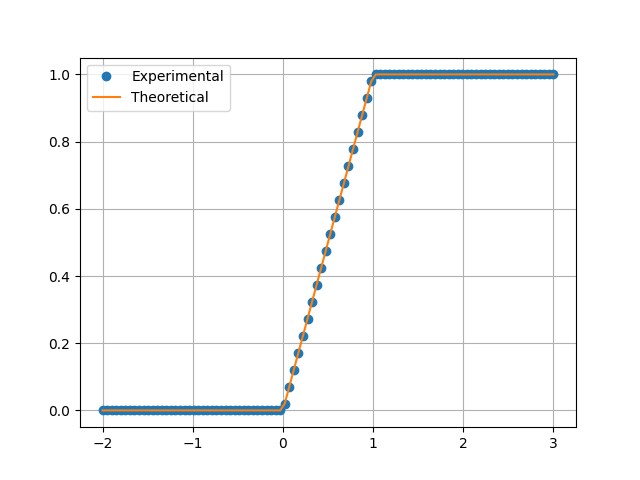
\includegraphics[width=\columnwidth]{figs/cdf_uni.png}
            \caption{CDF of $U$}
            \label{fig:cdf_uni}
        \end{figure}

    \item
        Find a theoretical expression for the CDF of $U$.
        \\
        \textbf{Solution}
        The PDF of $U$ is given by
        \begin{equation}
            p_U(x) = 
            \begin{cases}
                1 & 0 \leq x \leq 1 \\
                0 & \text{otherwise}
            \end{cases} \label{eq:pu}
        \end{equation}
        And so we can find the CDF,
        \begin{align}
            F_U(x) &= \int_{-\infty}^{x}{p_U(x) dx} \\
            F_U(x) &=
            \begin{cases}
                0 & x < 0 \\
                x & 0 \leq x \leq 1 \\
                1 & x > 1
            \end{cases} \label{eq:fu}
        \end{align}

    \item
        Write a C program to find the mean and variance of $U$.
        \\
        \textbf{Solution} Download the following files.
        \begin{lstlisting}
wget https://raw.githubusercontent.com/kst164/AI1110-Assignments/main/rand_nums/codes/mean_var.c
wget https://raw.githubusercontent.com/kst164/AI1110-Assignments/main/rand_nums/codes/uni.dat
        \end{lstlisting}
        And run it using
        \begin{lstlisting}
cc mean_var.c
./a.out < uni.dat
        \end{lstlisting}
        It will give the output
        \begin{lstlisting}
Mean    : 0.499631
Variance: 0.083320
        \end{lstlisting}

    \item
        Verify your result theoretically given that
        \begin{equation}
            E\left[U^k\right] = \int_{-\infty}^{\infty}{x^k d F_U(x)}
        \end{equation}
        \\
        \textbf{Solution}
        We use the fact that
        \begin{equation}
            d F_U(x) = p_U(x) dx
        \end{equation}

        So from eq \eqref{eq:pu}, we have
        \begin{align}
            E\left[U^k\right] &= \int_{-\infty}^{+\infty}{x^k p_U(x) dx} \\
            &= \int_{0}^{1}{x^k dx} \\
            &= \left(\frac{x^{k+1}}{k+1}\right)\Big|_0^1 \\
            &= \frac{1}{k+1} \label{eq:ek}
        \end{align}

        Now using eq \eqref{eq:ek}, we can find the mean of $U$
        \begin{equation}
            \mu = E\left[U\right] = \frac{1}{2}
        \end{equation}
        and the variance
        \begin{align}
            \text{var}\left[U\right] &= E\left[U^2\right] - E\left[U\right]^2 \\
            &= \frac{1}{3} - \left(\frac{1}{2}\right)^2 \\
            &= \frac{1}{12} = 0.83333..
        \end{align}
        We see that the theoretical mean and variance match with the experimental values.

\end{enumerate}

\section{Central Limit Theorem}

Let $X$ be a random variable defined as

\begin{equation}
    X = \sum_{i=1}^{12}{U_i - 6}
\end{equation}

\begin{enumerate}[label=\arabic{section}.\arabic*]
    \item
        Generate $10^6$ samples of X using a C program, and save into a file called gau.dat
        \\
        \textbf{Solution} Download the following C file.
        \begin{lstlisting}
wget https://raw.githubusercontent.com/kst164/AI1110-Assignments/main/rand_nums/codes/gen_gaussian.c
        \end{lstlisting}
        And run it using
        \begin{lstlisting}
cc gen_gaussian.c
./a.out > gau.dat
        \end{lstlisting}

    \item
        Load the gau.dat file into python and plot the empirical CDF of $X$ using the samples in gau.dat.
        What properties does the CDF have?
        \\
        \textbf{Solution} Download the following files.
        \begin{lstlisting}
wget https://raw.githubusercontent.com/kst164/AI1110-Assignments/main/rand_nums/codes/cdf_gau.py
wget https://raw.githubusercontent.com/kst164/AI1110-Assignments/main/rand_nums/codes/gau.dat
        \end{lstlisting}
        And run it using
        \begin{lstlisting}
python3 cdf_gau.py
        \end{lstlisting}
        It will generate the plot in Figure \eqref{fig:cdf_gau}.
        \begin{figure}[!ht]
            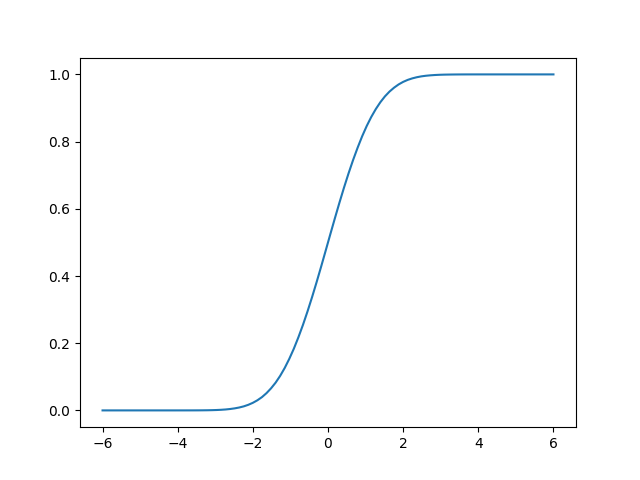
\includegraphics[width=\columnwidth]{figs/cdf_gau.png}
            \caption{CDF of $X$}
            \label{fig:cdf_gau}
        \end{figure}
        \\
        Properties of the CDF:
        \begin{itemize}
            \item $\lim\limits_{x \to -\infty} F_X(x) = 0$
            \item $\lim\limits_{x \to \infty} F_X(x) = 1$
            \item $F_X(0) = \frac{1}{2}$
            \item $F_X(x) + F_X(-x) = 1$
        \end{itemize}

    \item
        Load the gau.dat file into python and plot the empirical PDF of $X$ using the samples in gau.dat.
        What properties does the PDF have?
        \\
        \textbf{Solution} Download the following files.
        \begin{lstlisting}
wget https://raw.githubusercontent.com/kst164/AI1110-Assignments/main/rand_nums/codes/pdf_gau.py
wget https://raw.githubusercontent.com/kst164/AI1110-Assignments/main/rand_nums/codes/gau.dat
        \end{lstlisting}
        And run it using
        \begin{lstlisting}
python3 pdf_gau.py
        \end{lstlisting}
        It will generate the plot in Figure \eqref{fig:pdf_gau}.
        \begin{figure}[!ht]
            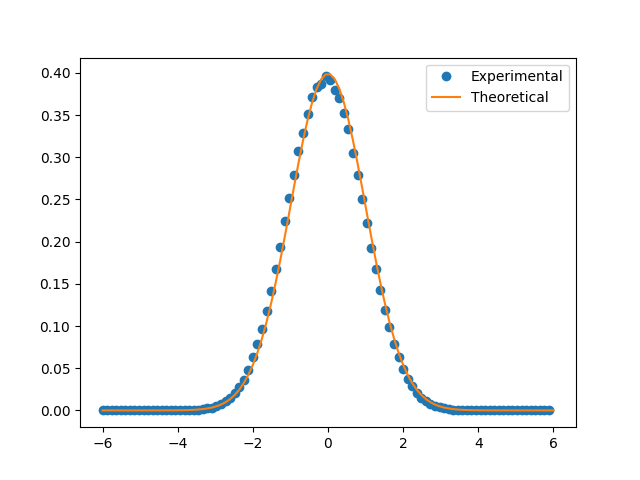
\includegraphics[width=\columnwidth]{figs/pdf_gau.png}
            \caption{PDF of $X$}
            \label{fig:pdf_gau}
        \end{figure}
        \\
        Properties of the PDF:
        \begin{itemize}
            \item $F_X(x) = F_X(-x)$ i.e., symmetric about 0
            \item PDF is bell shaped
            \item Peak of PDF is also the mean
        \end{itemize}

    \item
        Write a C program to find the mean and variance of $X$.
        \\
        \textbf{Solution} Download the following files.
        \begin{lstlisting}
wget https://raw.githubusercontent.com/kst164/AI1110-Assignments/main/rand_nums/codes/mean_var.c
wget https://raw.githubusercontent.com/kst164/AI1110-Assignments/main/rand_nums/codes/gau.dat
        \end{lstlisting}
        And run it using
        \begin{lstlisting}
cc mean_var.c
./a.out < gau.dat
        \end{lstlisting}
        It will give the output
        \begin{lstlisting}
Mean    : 0.000635
Variance: 0.999490
        \end{lstlisting}

    \item
        Given that
        \begin{equation}
            p_X(x) = \frac{1}{\sqrt{2 \pi}} \exp \left(-\frac{x^2}{2}\right)
        \end{equation}
        repeat the above exercise theoretically.
        \\
        \textbf{Solution}
        The mean is given by
        \begin{align}
            E\left[X\right] &= \int_{-\infty}^{\infty}{x p_X(x) dx} \\
            &= \int_{-\infty}^{\infty}{\frac{x}{\sqrt{2 \pi}} \exp\left(-\frac{x^2}{2}\right) dx}
        \end{align}
        Since this is the integral of an odd function over an odd interval, and the function goes to zero as $x$ diverges,
        \begin{equation}
            E\left[U\right] = 0
        \end{equation}

        To calculate variance of $X$
        \begin{align}
            \text{var}(X) &= E\left[X - E[X]\right]^2 \\
            &= E\left[X^2\right] \\
            &= \int_{-\infty}^{\infty}{x^2 p_X(x) dx} \\
            &= \int_{-\infty}^{\infty}{\frac{x^2}{\sqrt{2 \pi}} e^{-\frac{x^2}{2}} dx} \\
            &= \frac{1}{\sqrt{2 \pi}} \int_{-\infty}^{\infty}{x \cdot x e^{-\frac{x^2}{2}} dx}
        \end{align}

        Integrating by parts, we get
        \begin{align}
            \begin{split}
            \text{var}(X) &= \frac{1}{\sqrt{2 \pi}}\Bigg(-x \text{exp}\left(\frac{-x^2}{2}\right) \\
            &+ \int{\text{exp}\left(\frac{-x^2}{2}\right) dx}\Bigg) \Bigg|_{-\infty}^{\infty}
            \end{split}
            \\
            &= \frac{1}{\sqrt{2 \pi}} \int_{-\infty}^{\infty}{\text{exp}\left(\frac{-x^2}{2}\right) dx} \\
        \end{align}
        Substituting the Gaussian integral,
        \begin{equation}
            \text{var}(X) = 1
        \end{equation}

\end{enumerate}

\section{From Uniform to Other}

\begin{enumerate}[label=\arabic{section}.\arabic*]
    \item
        Generate samples of
        \begin{equation}
            V = -2 \ln(1 - U)
        \end{equation}
        and plot its CDF
        \\
        \textbf{Solution} Download the following files.
        \begin{lstlisting}
wget https://raw.githubusercontent.com/kst164/AI1110-Assignments/main/rand_nums/codes/cdf_v.py
wget https://raw.githubusercontent.com/kst164/AI1110-Assignments/main/rand_nums/codes/uni.dat
        \end{lstlisting}
        And run it using
        \begin{lstlisting}
python3 cdf_v.py
        \end{lstlisting}
        It will generate the plot in Figure \eqref{fig:cdf_v}.
        \begin{figure}[!ht]
            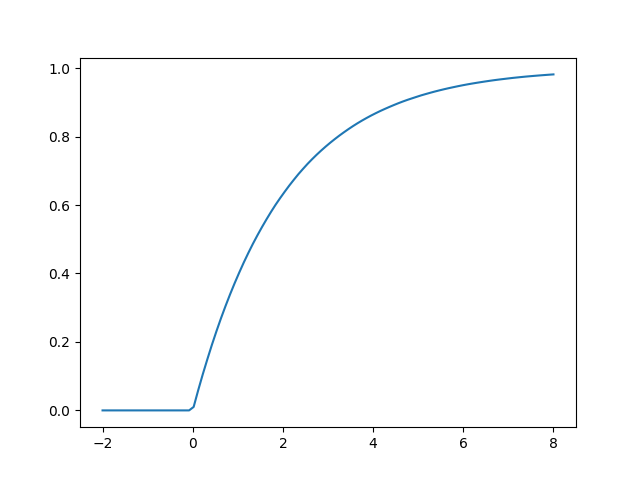
\includegraphics[width=\columnwidth]{figs/cdf_v.png}
            \caption{CDF of $V$}
            \label{fig:cdf_v}
        \end{figure}

    \item
        Find a theoretical expression for $F_V(x)$
        \\
        \textbf{Solution}
        \begin{align}
            F_V(x) &= \pr{x \leq V} \\
            &= \pr{x \leq -2 \log (1 - U)} \\
            &= \pr{\log (1 - U) \leq \frac{-x}{2}} \\
            &= \pr{1 - U \leq \exp \left(\frac{-x}{2}\right)} \\
            &= \pr{1 - \exp \left(\frac{-x}{2}\right) \leq U} \\
            &= F_U \left(1 - \exp \left(\frac{-x}{2}\right)\right)
        \end{align}

        We know $F_U(x)$ from eq \eqref{eq:fu}, so we have
        \begin{align}
            F_V(x) &= F_U \left(1 - \exp \left(\frac{-x}{2}\right)\right) \\
            &= \begin{cases}
                0 & 1 - e^{\frac{-x}{2}} < 0 \\
                1 - e^{\frac{-x}{2}} & 0 < 1 - e^{\frac{-x}{2}} < 1 \\
                1 & 1 - e^{\frac{-x}{2}} > 1
            \end{cases}
        \end{align}
        Simplifying, we get
        \begin{equation}
            F_V(x) = \begin{cases}
                0 & x < 0 \\
                1 - \exp \left(\frac{-x}{2}\right) & x \geq 0
            \end{cases}
        \end{equation}
\end{enumerate}

\section{Triangular Distribution}

\begin{enumerate}[label=\arabic{section}.\arabic*]
    \item
        Generate
        \begin{equation}
            T = U_1 + U_2
        \end{equation}
        \\
        \textbf{Solution} Download the following C file.
        \begin{lstlisting}
wget https://raw.githubusercontent.com/kst164/AI1110-Assignments/main/rand_nums/codes/gen_triangular.c
        \end{lstlisting}
        And run it using
        \begin{lstlisting}
cc gen_triangular.c
./a.out > tri.dat
        \end{lstlisting}

    \item
        Find the CDF of $T$
        \\
        \textbf{Solution} Download the following files.
        \begin{lstlisting}
wget https://raw.githubusercontent.com/kst164/AI1110-Assignments/main/rand_nums/codes/cdf_tri_num.py
wget https://raw.githubusercontent.com/kst164/AI1110-Assignments/main/rand_nums/codes/tri.dat
        \end{lstlisting}
        And run it using
        \begin{lstlisting}
python3 cdf_tri_num.py
        \end{lstlisting}
        It will generate the plot in Figure \eqref{fig:cdf_tri_num}.
        \begin{figure}[!ht]
            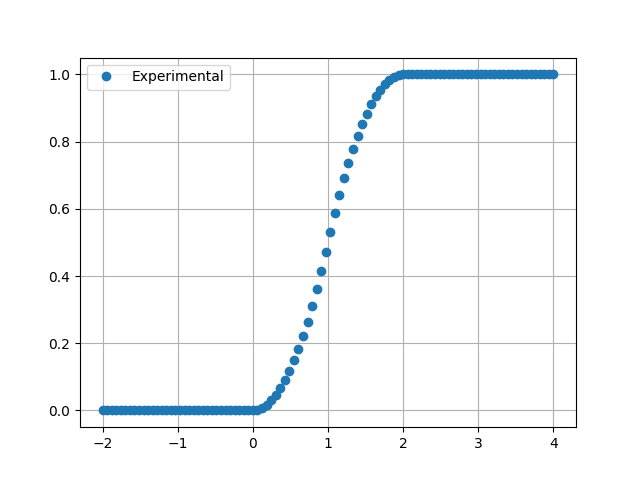
\includegraphics[width=\columnwidth]{figs/cdf_tri_num.png}
            \caption{Experimental CDF of V}
            \label{fig:cdf_tri_num}
        \end{figure}

    \item
        Find the PDF of $T$
        \\
        \textbf{Solution} Download the following files
        \begin{lstlisting}
wget https://raw.githubusercontent.com/kst164/AI1110-Assignments/main/rand_nums/codes/pdf_tri_num.py
wget https://raw.githubusercontent.com/kst164/AI1110-Assignments/main/rand_nums/codes/tri.dat
        \end{lstlisting}
        And run it using
        \begin{lstlisting}
python3 pdf_tri_num.py
        \end{lstlisting}
        It will generate the plot in Figure \eqref{fig:pdf_tri_num}.
        \begin{figure}[!ht]
            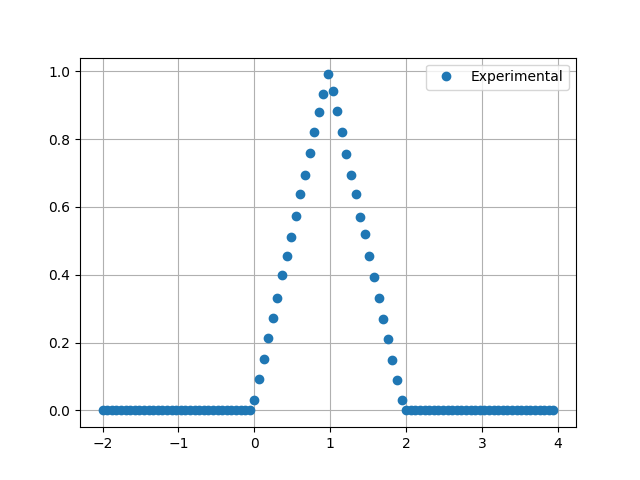
\includegraphics[width=\columnwidth]{figs/pdf_tri_num.png}
            \caption{Experimental PDF of $X$}
            \label{fig:pdf_tri_num}
        \end{figure}

    \item
        Find the theoretical expressions for the CDF and PDF of $T$
        \\
        \textbf{Solution}
        \begin{equation}
            T = U_1 + U_2
        \end{equation}
        So we have
        \begin{equation}
            p_T(t) = (p_{U_1} * p_{U_2})(t)
        \end{equation}
        Since $U_1$ and $U_2$ are i.i.d., $p_{U_1}(t)=p_{U_2}(t)=p_U(t)$, which is given by eq \eqref{eq:pu}.
        \begin{equation}
            p_T(t) = \int_{-\infty}^{\infty}p_U(\tau)p_U(t - \tau) d\tau
        \end{equation}
        When $\tau<0$ or $\tau>1$, the integral evaluates to 0.
        \begin{align}
            p_T(t) &= \int_{0}^{1}p_U(\tau)p_U(t - \tau) d\tau \\
                   &= \int_{0}^{1}p_U(t - \tau) d\tau
        \end{align}
        When $t<0$ or $t>2$, the integral evaluates to 0. When $0<t<1$,
        \begin{align}
            p_T(t) &= \int_{0}^{1}p_U(t - \tau) d\tau \\
                   &= \int_{0}^{t} d\tau + \int_{t}^{1}0 \cdot d\tau \\
                   &= t
        \end{align}
        When $1<t<2$,
        \begin{align}
            p_T(t) &= \int_{0}^{1}p_U(t - \tau) d\tau \\
                   &= \int_{0}^{t-1}0 \cdot d\tau + \int_{t-1}^{1} d\tau \\
                   &= 2 - t
        \end{align}
        Therefore the PDF is
        \begin{equation}
            p_T(t) = \begin{cases}
                0 & t < 0 \\
                t & 0 < t < 1 \\
                2 - t & 1 < t < 2 \\
                0 & t > 2
            \end{cases}
        \end{equation}
        The CDF of $T$ is given by
        \begin{equation}
            F_T(t) = \int_{0}^{t}p_T(t)dt
        \end{equation}
        Simplifying, we get
        \begin{equation}
            F_T(t) = \begin{cases}
                0 & t < 0 \\
                \frac{t^2}{2} & 0 < t < 1 \\
                -\frac{t^2}{2} + 2t - 1 & 1 < t < 2 \\
                1 & t > 2
            \end{cases}
        \end{equation}

    \item
        Verify your results through a plot
        \\
        \textbf{Solution} Download the following files
        \begin{lstlisting}
wget https://raw.githubusercontent.com/kst164/AI1110-Assignments/main/rand_nums/codes/pdf_tri.py
wget https://raw.githubusercontent.com/kst164/AI1110-Assignments/main/rand_nums/codes/cdf_tri.py
wget https://raw.githubusercontent.com/kst164/AI1110-Assignments/main/rand_nums/codes/tri.dat
        \end{lstlisting}
        And run them using
        \begin{lstlisting}
python3 pdf_tri.py
python3 cdf_tri.py
        \end{lstlisting}
        They will generate the plots in Figures \eqref{fig:cdf_tri} and \eqref{fig:pdf_tri}.
        \begin{figure}[!ht]
            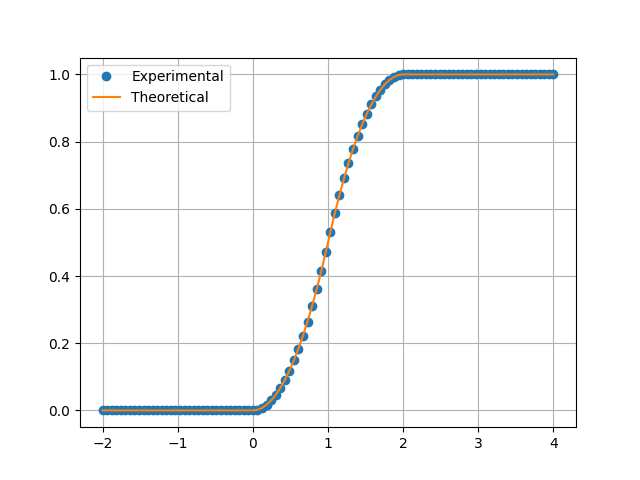
\includegraphics[width=\columnwidth]{figs/cdf_tri.png}
            \caption{CDF of $X$}
            \label{fig:cdf_tri}
        \end{figure}
        \begin{figure}[!ht]
            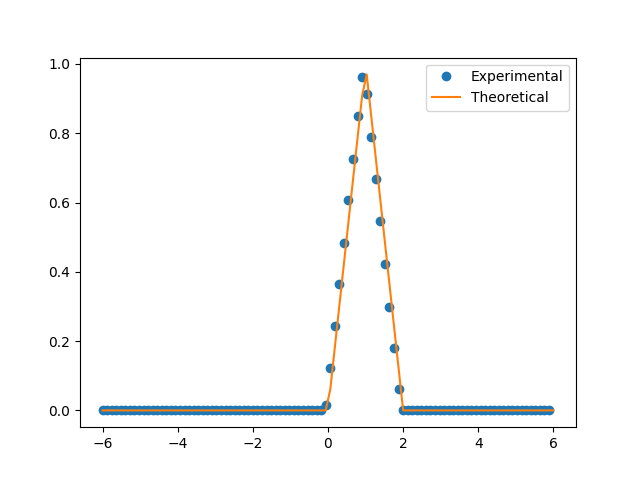
\includegraphics[width=\columnwidth]{figs/pdf_tri.png}
            \caption{PDF of $X$}
            \label{fig:pdf_tri}
        \end{figure}

\end{enumerate}

\section{Maximum Likelihood}

\begin{enumerate}[label=\arabic{section}.\arabic*]
    \item
        Generate equiprobable $X \in \{1, -1\}$.
        \\
        \textbf{Solution} Download the following C file
        \begin{lstlisting}
wget https://raw.githubusercontent.com/kst164/AI1110-Assignments/main/rand_nums/codes/gen_bernoulli.c
        \end{lstlisting}
        And run it using
        \begin{lstlisting}
cc gen_bernoulli.c
./a.out > ber.dat
        \end{lstlisting}

    \item
        Generate
        \begin{equation}
            Y = AX + N
        \end{equation}
        where $A$ = 5 dB, and $ N \sim \mathcal{N}(0, 1)$.
        \\
        \textbf{Solution} Download the following files
        \begin{lstlisting}
wget https://raw.githubusercontent.com/kst164/AI1110-Assignments/main/rand_nums/codes/gen_y.py
        \end{lstlisting}
        And run it using
        \begin{lstlisting}
python gen_y.py
        \end{lstlisting}
        It will create the file \texttt{maxlike.dat} containing $Y$.

    \item
        Plot $Y$ using a scatter plot.
        \\
        \textbf{Solution} Download the following files
        \begin{lstlisting}
wget https://raw.githubusercontent.com/kst164/AI1110-Assignments/main/rand_nums/codes/scatter_y.py
wget https://raw.githubusercontent.com/kst164/AI1110-Assignments/main/rand_nums/codes/maxlike.dat
        \end{lstlisting}
        And run it using
        \begin{lstlisting}
python scatter_y.py
        \end{lstlisting}
        It will generate the plot in Figure \eqref{fig:scatter_y}.
        \begin{figure}[!ht]
            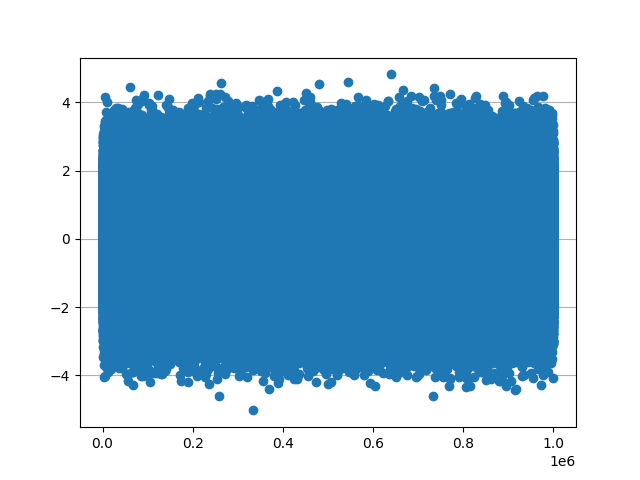
\includegraphics[width=\columnwidth]{figs/scatter_y.png}
            \caption{Scatter plot of $Y$}
            \label{fig:scatter_y}
        \end{figure}

    \item
        Guess how to estimate $X$ from $Y$.
        \\
        \textbf{Solution} We can estimate $X$ using
        \begin{equation}
            \hat{X} = \begin{cases}
                1 & Y \geq 0 \\
                -1 & Y < 0
            \end{cases}
        \end{equation}

    \item
        Find
        \begin{equation}
            P_{e|0} = \pr{\hat{X} = -1 | X = 1}
        \end{equation}
        and
        \begin{equation}
            P_{e|1} = \pr{\hat{X} = 1 | X = 0}
        \end{equation}
        \\
        \textbf{Solution} We have
        \begin{align}
            P_{e|0} &= \pr{\hat{X} = -1 | X = 1} \\
            &= \pr{AX + N < 0 | X = 1} \\
            &= \pr{A + N < 0} \\
            &= \pr{N < -A} \\
            &= F_N(-A) \\
            &= Q(A)
        \end{align}
        and
        \begin{align}
            P_{e|1} &= \pr{\hat{X} = 1 | X = -1} \\
            &= \pr{AX + N \geq 0 | X = -1} \\
            &= \pr{-A + N \geq 0} \\
            &= \pr{N \geq A} \\
            &= Q(A)
        \end{align}
        So we have our result
        \begin{equation}
            P_{e|0} = P_{e|1} = Q(A)
        \end{equation}

    \item
        Find $P_e$ assuming $X$ has equiprobable symbols
        \\
        \textbf{Solution} We need to find
        \begin{align}
        \begin{split}
            P_e &= P_{e|0} \cdot \pr{X = -1} \\
            &\quad+ P_{e|1} \cdot \pr{X = 1}
        \end{split} \\
            &= Q(A) \cdot \frac{1}{2} + Q(A) \cdot \frac{1}{2} \\
            P_e &= Q(A)
        \end{align}

    \item
        Verify by plotting the theoretical $P_e$ with respect to $A$ from 0 to 10 dB
        \\
        \textbf{Solution} Download the following files
        \begin{lstlisting}
wget https://raw.githubusercontent.com/kst164/AI1110-Assignments/main/rand_nums/codes/error_ml.py
wget https://raw.githubusercontent.com/kst164/AI1110-Assignments/main/rand_nums/codes/ber.dat
wget https://raw.githubusercontent.com/kst164/AI1110-Assignments/main/rand_nums/codes/gau.dat
        \end{lstlisting}
        And run it using
        \begin{lstlisting}
python error_ml.py
        \end{lstlisting}
        It will generate the plot in Figure \eqref{fig:error_ml}.
        \begin{figure}[!ht]
            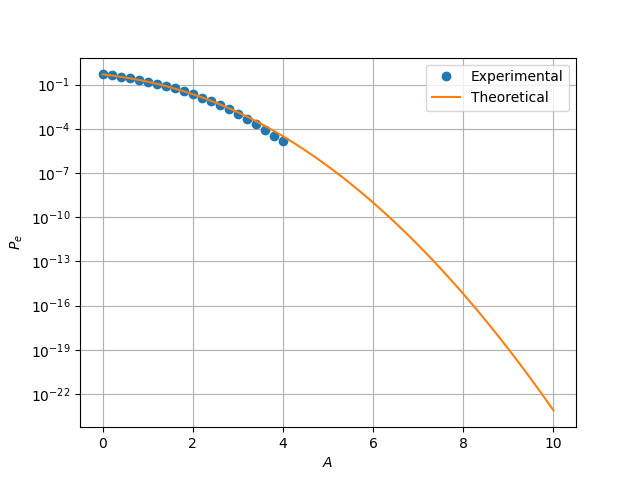
\includegraphics[width=\columnwidth]{figs/error_ml.png}
            \caption{semilog plot of $P_e$}
            \label{fig:error_ml}
        \end{figure}

    \item
        Now, consider a threshold $\delta$ while estimating $X$ from $Y$. Find the value of $\delta$
        that maximizes the theoretical $P_e$.
        \\
        \textbf{Solution} We can define our guess as
        \begin{equation}
            \hat{X} = \begin{cases}
                1 & Y \geq \delta \\
                -1 & Y < \delta
            \end{cases}
        \end{equation}
        Now,
        \begin{align}
            P_{e|0} &= \pr{\hat{X} = -1 | X = 1} \\
            &= \pr{AX + N < \delta | X = 1} \\
            &= \pr{A + N < \delta} \\
            &= \pr{N < -A + \delta} \\
            &= F_N(-(A - \delta)) \\
            &= Q(A - \delta)
        \end{align}
        And similarly,
        \begin{equation}
            P_{e|1} = Q(A + \delta)
        \end{equation}
        So we have,
        \begin{align}
        \begin{split}
            P_e &= P_{e|0} \cdot \pr{X = -1} \\
            &\quad+ P_{e|1} \cdot \pr{X = 1}
        \end{split} \\
            &= Q(A - \delta) \cdot \frac{1}{2} + Q(A + \delta) \cdot \frac{1}{2} \label{eq:p_e}
        \end{align}
        To find the minimal $P_e$, we differentiate Eq \eqref{eq:p_e} wrt $\delta$ and equate it to
        0
        \begin{align}
            0 &= \frac{d}{d\delta}\left(\frac{1}{2}\left(Q(A-\delta) + Q(A+\delta)\right)\right) \\
            &= \frac{1}{2} \frac{1}{\sqrt{2\pi}}
                \left(e^{-\frac{(A-\delta)^2}{2}} - e^{-\frac{(A+\delta)^2}{2}}\right)
        \end{align}
        So we have
        \begin{align}
            (A - \delta)^2 &= (A + \delta)^2 \\
            \implies \delta &= 0
        \end{align}
        So $P_e$ is minimal when the threshold is $\delta = 0$.

    \item
        Repeat the above exercise when
        \begin{equation}
            p_X(0) = p
        \end{equation}
        \\
        \textbf{Solution} We have
        \begin{align}
            P_e &= P_{e|0} p + P_{e|1} (1 - p) \\
            &= Q(A - \delta) p + Q(A + \delta) (1 - p)
        \end{align}
        Differentiating wrt $\delta$ to get minimum,
        \begin{align}
            0 &= \frac{d}{d\delta}(Q(A - \delta) p + Q(A + \delta) (1 - p)) \\
            &= pe^{-\frac{(A - \delta)^2}{2}} - (1 - p) e^{-\frac{(A + \delta)^2}{2}}
        \end{align}
        Taking $\ln$,
        \begin{align}
            \ln{p} - \frac{(A - \delta)^2}{2} &= \ln(1 - p) - \frac{(A + \delta)^2}{2} \\
            2 A \delta &= \ln \frac{1 - p}{p} \\
            \delta &= \frac{1}{2 A} \ln \frac{1 - p}{p}
        \end{align}
        And so we have our result

    \item
        Repeat the above exercise using the MAP criterion.
        \\
        \textbf{Solution}
        Assume $\pr{X = -1} = p$.

        According to the MAP criterion, when
        \begin{equation}
            p_{X|Y}(-1|y) > p_{X|Y}(1|y) \label{eq:5.10:MAP}
        \end{equation}
        We should guess -1, else we guess 1. Now,
        \begin{equation}
            p_{X|Y}(x|y) = \frac{p_{Y|X}(y|x)p_X(x)}{p_Y(y)} \label{eq:5.10:x|y}
        \end{equation}
        %To find $p_Y(y)$
        %\begin{align}
        %\begin{split}
            %p_{Y}(y) &= p_{Y|X}(y|-1)(p) \\
            %&\quad+ p_{Y|X}(y|1)(1 - p)
        %\end{split}
        %\end{align}
        Now,
        \begin{equation}
            p_{Y|X}(y|-1) = p_{(-A+N)}(y)
        \end{equation}
        Since $A$ is a constant,
        \begin{align}
            p_{Y|X}(y|-1) &= p_{N}(y + A) \\
            &= \frac{1}{\sqrt{2 \pi}}e^{-\frac{(y + A)^2}{2}}
        \end{align}
        Substituting into \eqref{eq:5.10:x|y},
        \begin{align}
            p_{X|Y}(-1|y) &= \frac{p_{Y|X}(y|-1)p_X(-1)}{p_Y(y)} \\
            p_{X|Y}(-1|y) &= \frac{\frac{1}{\sqrt{2 \pi}} e^{-\frac{(y+A)^2}{2}} p}{p_Y(y)}
                \label{eq:5.10:-1|y}
        \end{align}
        Similarly,
        \begin{align}
            p_{X|Y}(1|y) &= \frac{\frac{1}{\sqrt{2 \pi}} e^{-\frac{(y-A)^2}{2}} (1-p)}{p_Y(y)}
                \label{eq:5.10:1|y}
        \end{align}
        Finally, substituting Eqs \eqref{eq:5.10:-1|y} and \eqref{eq:5.10:1|y} into Eq
        \eqref{eq:5.10:MAP}, we should guess that $X = -1$ when
        \begin{align}
            \frac{\frac{1}{\sqrt{2 \pi}} e^{-\frac{(y+A)^2}{2}} p}{p_Y(y)}
                &> \frac{\frac{1}{\sqrt{2 \pi}} e^{-\frac{(y-A)^2}{2}} (1-p)}{p_Y(y)} \\
            \frac{p}{1-p} &> e^{2 A y} \\
            y &< \frac{1}{2A} \ln \frac{p}{1-p}
        \end{align}
        And so we have our guess,
        \begin{equation}
            \hat{X} = \begin{cases}
                -1 & y < \delta \\
                1 & \text{otherwise}
            \end{cases}
        \end{equation}
        where $\delta = \frac{1}{2A} \ln \frac{p}{1-p}$.

        Consider the special case $p=\frac{1}{2}$
        \begin{align}
            \delta &= \frac{1}{2 A} \ln 1 \\
            \delta &= 0
        \end{align}
        So our guess is,
        \begin{equation}
            \hat{X} = \begin{cases}
                -1 & y < 0 \\
                1 & y > 0
            \end{cases}
        \end{equation}

\end{enumerate}

\section{Gaussian to Other}

\begin{enumerate}[label=\arabic{section}.\arabic*]
    \item
        Let $X_1 \sim \mathcal{N}(0, 1)$ and $X_1 \sim \mathcal{N}(0, 1)$. Plot the CDF and PDF of
        \begin{equation}
            V = X_1^2 + X_2^2
        \end{equation}
        \\
        \textbf{Solution} Download the following files.
        \begin{lstlisting}
wget https://raw.githubusercontent.com/kst164/AI1110-Assignments/main/rand_nums/codes/cdf_chi.py
wget https://raw.githubusercontent.com/kst164/AI1110-Assignments/main/rand_nums/codes/pdf_chi.py
wget https://raw.githubusercontent.com/kst164/AI1110-Assignments/main/rand_nums/codes/chi.dat
        \end{lstlisting}
        And run them using
        \begin{lstlisting}
python3 cdf_chi.py
python3 pdf_chi.py
        \end{lstlisting}
        They will generate the plots in Figures \eqref{fig:cdf_chi} and \eqref{fig:pdf_chi}.
        \begin{figure}[!ht]
            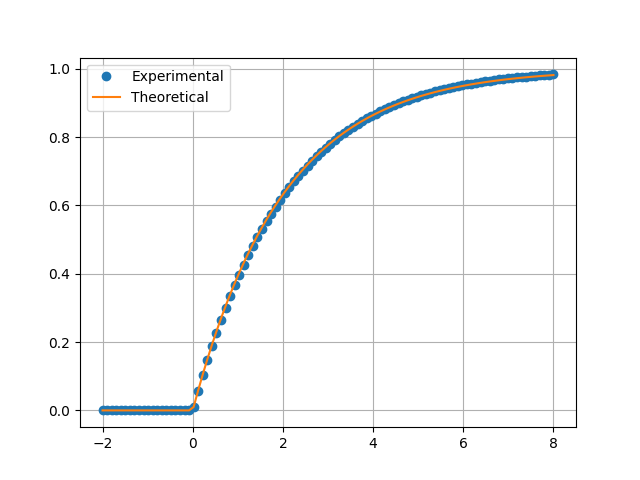
\includegraphics[width=\columnwidth]{figs/cdf_chi.png}
            \caption{CDF of $V$}
            \label{fig:cdf_chi}
        \end{figure}
        \begin{figure}[!ht]
            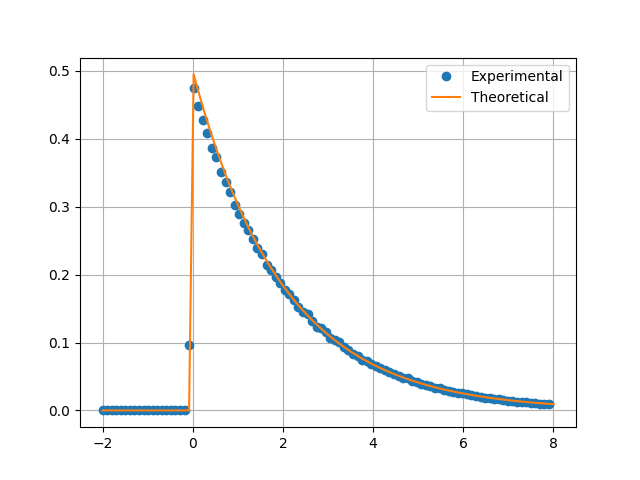
\includegraphics[width=\columnwidth]{figs/pdf_chi.png}
            \caption{PDF of $V$}
            \label{fig:pdf_chi}
        \end{figure}

    \item
        If
        \begin{equation}
            F_V(x) = \begin{cases}
                1 - e^{- \alpha x} & x \geq 0 \\
                0 & x < 0
            \end{cases}
        \end{equation}
        Find $\alpha$.
        \\
        \textbf{Solution} We define the random variables
        \begin{align}
            X_1 = R \cos \Theta \\
            X_2 = R \sin \Theta
        \end{align}
        The Jacobian matrix is given by
        \begin{align}
            J &= \begin{bmatrix}
                \frac{\partial X_1}{\partial R} & \frac{\partial X_1}{\partial \Theta} \\
                \frac{\partial X_2}{\partial R} & \frac{\partial X_2}{\partial \Theta}
            \end{bmatrix} \\
            J &= \begin{bmatrix}
                \cos \Theta & -R \sin \Theta \\
                \sin \Theta & R \cos \Theta
            \end{bmatrix} \\
            \implies |J| &= R \label{eq:6.2:jacobian}
        \end{align}
        Also, since $X_1$ and $X_2$ are iid,
        \begin{align}
            p_{X1,X2}(x_1, x_2) &= p_{X_1}(x_1) p_{X_2}(x_2) \\
            &= \frac{1}{2 \pi}e^{-\frac{x_1^2 + x_2^2}{2}} \\
            &= \frac{1}{2 \pi}e^{-\frac{r^2}{2}} \label{eq:6.2:px1x2}
        \end{align}
        Now since
        \begin{equation}
            p_{R, \Theta}(r, \theta) = |J| p_{X_1, X_2}(x_1, x_2)
        \end{equation}
        From Eqs \eqref{eq:6.2:jacobian} and \eqref{eq:6.2:px1x2}, we have
        \begin{align}
            p_{R, \Theta}(r, \theta) &= \frac{r}{2 \pi}e^{-\frac{r^2}{2}} \\
            \implies p_{R}(r) &= \int_{0}^{2 \pi} p_{R, \Theta}(r, \theta) d \theta \\
            &= r e^{-{\frac{r^2}{2}}}
        \end{align}
        We then have
        \begin{align}
            F_R(r) &= \int_{0}^{r} p_R(r) \\
            &= \int_{0}^{r} r e^{-\frac{r^2}{2}} dr \\
            &= \left(-e^{-\frac{r^2}{2}}\right)_{0}^{r} \\
            &= 1 - e^{-\frac{r^2}{2}}
        \end{align}
        Finally,
        \begin{align}
            F_V(x) &= \pr{V \leq x} \\
            &= \pr{X_1^2 + X_2^2 \leq x} \\
            &= \pr{R^2 \leq x}
            &= \pr{R \leq \sqrt{x}} \\
            &= F_R(\sqrt{x}) \\
            &= 1 - e^{-\frac{x}{2}} \\
            &= 1 - e^{- \alpha x}
        \end{align}
        And so we have our result
        \begin{equation}
            \alpha = \frac{1}{2}
        \end{equation}

    \item
        Plot the CDF and PDF of
        \begin{equation}
            A = \sqrt{V}
        \end{equation}
        \\
        \textbf{Solution} Download the following files.
        \begin{lstlisting}
wget https://raw.githubusercontent.com/kst164/AI1110-Assignments/main/rand_nums/codes/cdf_ray.py
wget https://raw.githubusercontent.com/kst164/AI1110-Assignments/main/rand_nums/codes/pdf_ray.py
wget https://raw.githubusercontent.com/kst164/AI1110-Assignments/main/rand_nums/codes/chi.dat
        \end{lstlisting}
        And run them using
        \begin{lstlisting}
python3 cdf_ray.py
python3 pdf_ray.py
        \end{lstlisting}
        They will generate the plots in Figures \eqref{fig:cdf_ray} and \eqref{fig:pdf_ray}.
        \begin{figure}[!ht]
            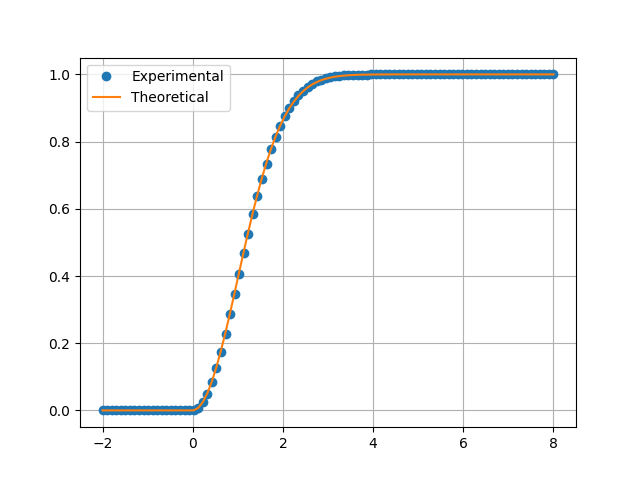
\includegraphics[width=\columnwidth]{figs/cdf_ray.png}
            \caption{CDF of $V$}
            \label{fig:cdf_ray}
        \end{figure}
        \begin{figure}[!ht]
            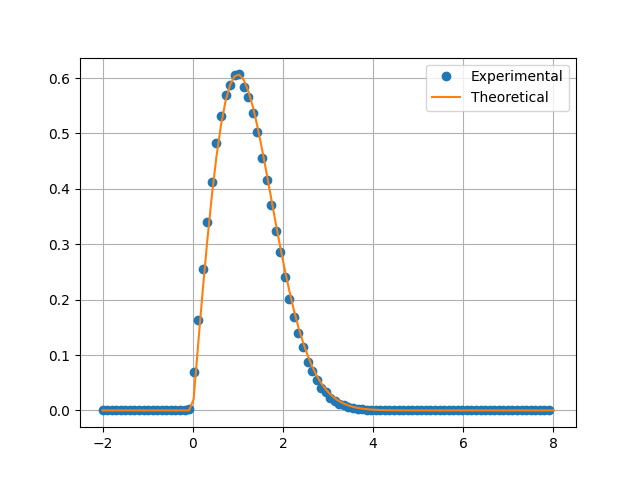
\includegraphics[width=\columnwidth]{figs/pdf_ray.png}
            \caption{PDF of $V$}
            \label{fig:pdf_ray}
        \end{figure}

\end{enumerate}

\end{document}
